\documentclass[conference]{IEEEtran}
\usepackage[utf8]{inputenc}
\usepackage{graphicx}
\usepackage{amsmath}
\usepackage{hyperref}
\usepackage{cite}

\title{TempCon-RingCast: Temperature and Congestion-Aware Multicast Communication in Ring-Based Optical Network-on-Chip (ONoC)}

\author{
    \IEEEauthorblockN{Abubeker Yasmin Mustefa\IEEEauthorrefmark{1}}
    \IEEEauthorblockA{\IEEEauthorrefmark{1}Department of Computer science, China Three Gorges University, Yichang , China\\
    Email: moli614360@gmail.com}
}

\date{\today}

\begin{document}

\maketitle

\begin{abstract}
This paper addresses the critical challenges of temperature and congestion in ring-based Optical Network-on-Chip (ONoC). As the demand for high-performance, energy-efficient interconnect systems grows, thermal management and congestion reduction have become essential for scalable and reliable multi-core processors. This study proposes a routing approach tailored for multicast communication, which utilizes a temperature-aware heuristic routing algorithm and congestion monitoring system, calibrated to respond dynamically to real-time network conditions. Experimental results demonstrate that this approach optimally balances temperature distribution and reduces congestion within the ONoC, thus enhancing the network efficiency and reliability. These findings have significant implications for industries reliant on efficient data processing and transfer, such as artificial intelligence, cloud computing, and big data analytics, where ONoC are crucial for meeting the increasing demands for high-performance computing and low-latency communication. Furthermore, advancements in ONoC technology directly impact the development of next-generation processors and computing systems, enabling more complex and computationally intensive applications.
\end{abstract}

\section{Introduction}
Optical Network-on-Chip (ONoC) has emerged as a promising alternative to traditional electrical interconnects, offering superior bandwidth, reduced latency, and lower power consumption. The increasing integration density within ONoC presents significant challenges in thermal management and network congestion. Ring-based topology, frequently favored for their simplicity and scalability, faces particular thermal management challenges. The closed-loop structure and constant traffic circulation in these topologies can generate localized hot-spots, leading to system reliability issues. Additionally, the ring structure creates potential congestion bottlenecks that can significantly impact network performance.

Recent advances in temperature-aware and congestion-aware routing algorithms have made progress in addressing thermal and congestion challenges. Temperature-aware strategies optimize routing based on thermal profiles to maintain system reliability. Concurrently, congestion-aware routing strategies manage network load dynamically to maintain optimal performance. However, existing approaches often address these concerns independently, lacking a unified strategy for handling both temperature and congestion in the multicast ONoC environment \cite{li2021contention}.

In this paper, we propose an integrated approach called \textbf{TempCon-RingCast} that combines temperature-aware and congestion-aware routing into a single methodology, specifically targeting multicast communication in ring-based ONoC. By dynamically selecting paths based on real-time thermal and congestion data, the proposed method aims to enhance network performance and reliability. This approach is anticipated to benefit applications requiring efficient and stable data routing in ONoC, such as high-performance computing systems and data centers. The successful implementation of TempCon-RingCast can lead to more energy-efficient and reliable ONoC designs, which are essential for sustaining the growth and innovation in various technology sectors.

The rest of this paper is organized as follows: Section II describes the existing research results and progress in temperature and congestion management for ONoC, Section III presents our proposed TempCon-RingCast methodology and algorithms, Section IV evaluates the performance through comprehensive simulations and presents the analysis of results. Finally, the paper is concluded in Section V with a brief discussion of future research directions.

\section{Related Work}

\subsection{Temperature-Aware Routing}
Temperature management in ONoC has emerged as a critical challenge due to the increasing integration density and power consumption of modern chip designs. Recent research has focused on developing temperature-aware routing strategies to address these challenges. Smith et al. \cite{smith2020temperature} proposed a temperature-aware routing algorithm specifically designed for ring-based ONoC, demonstrating significant improvements in thermal distribution. Xie et al. \cite{xie2020thermal} introduced a message-passing based thermal-aware routing approach that achieved better temperature balance through dynamic path selection. Additionally, Li et al. \cite{li2021contention} developed a contention-aware routing scheme that considers both thermal reliability and network performance, showing that integrated approaches can better address thermal challenges.

\subsection{Congestion-Aware Routing}
Congestion management in ONoC has been extensively studied, with various approaches proposed to optimize network performance. Zhang et al. \cite{zhang2019congestion} presented a congestion-aware multicast routing algorithm that significantly reduced network bottlenecks. Li et al. \cite{li2018congestion} developed a comprehensive congestion-aware routing strategy that demonstrated improved throughput and reduced latency. The work by Wang et al. \cite{wang2019multicast} specifically addressed multicast routing challenges in ONoC, proposing algorithms that effectively balance network load while maintaining performance.

Existing research has largely focused on either temperature-aware or congestion-aware routing independently. However, these approaches often fall short in providing a holistic solution, as they fail to address the interplay between temperature and congestion. Few methods consider both aspects simultaneously, leaving a gap in addressing scenarios where both thermal and congestion issues exacerbate each other. To bridge this gap, we propose TempCon-RingCast, an integrated approach that dynamically selects paths based on real-time thermal and congestion data, aiming to enhance network performance and reliability by considering both factors concurrently.

\section{Proposed Methodology}
In the section, we propose a Temperature and Congestion-Aware Multicast Communication algorithm in Ring-Based Optical Network-on-Chip (called TempCon-RingCast), which integrates temperature and congestion awareness into the routing process to optimize network performance. The algorithm operates in several key steps: First, it measures temperature and congestion levels across the network. Second, it partitions the network to enable localized control. Third, it evaluates paths bidirectionally, and finally, it selects the optimal path based on a combined metric. The following subsections describe each step in detail.

\subsection{Temperature Measurement}
Temperature at each node and along each link is monitored using resonant wavelength shifts observed in the micro-ring resonators (MRs) \cite{bc972821a43d4cf989b222e9cdc15a79} associated with each network node. The shift in resonant wavelength (\(\Delta \lambda\)) serves as an indicator of temperature changes, which are calculated using the thermos-optic coefficient specific to the ONoC's material composition (e.g., silicon with a coefficient of \(1.86 \times 10^{-4} \, \mathrm{K}^{-1}\)).

The calculation involves the following steps:
\begin{itemize}
    \item \textbf{Wavelength Shift Measurement:} The resonant wavelength shift (\(\Delta \lambda\)) is measured through optical monitoring systems.
    \item \textbf{Temperature Calculation:} Using the formula
    \begin{equation}
    T = T_0 + \frac{\Delta \lambda}{\lambda_0 \cdot \alpha}
    \end{equation}
    where \(T_0\) is room temperature, and the system calculates the real-time temperature for each node.
\end{itemize}

\subsection{Congestion Measurement}
Congestion is quantified by assessing link utilization and traffic load at each node. The congestion metric for each link is calculated using the following equation:
\begin{equation}
    C_{\text{link}} = \frac{\text{Current Traffic Load}}{\text{Link Capacity}} \times 100\%
\end{equation}

The total path congestion is calculated as:
\begin{equation}
    C_{\text{path}} = \sum_{i=1}^{n} C_{\text{link}_i}
\end{equation}
where n is the number of links in the path.

\subsection{Path Partitioning}
Path partitioning is employed to manage temperature and congestion efficiently within the ring-based ONoC. By dividing the network into smaller, manageable partitions, the system achieves more granular control over temperature and congestion levels, reducing the complexity of the routing problem and allowing for more targeted management of network resources. This partitioned structure improves the accuracy of congestion and temperature measurements and simplifies routing decisions by enabling localized adjustments within each partition \cite{chen2020partitioning}.

\subsubsection{Partition Structure and Purpose}
Each partition is designed to contain approximately 5\% of the total nodes in the network, providing a balance between detailed monitoring and computational efficiency. For instance, in a network with 200 nodes, each partition would comprise 10 nodes. This layout allows for close monitoring of both thermal conditions and congestion in specific regions, enabling localized responses to emerging hot-spots or congestion points \cite{liu2019wavelength}. By isolating regions in this manner, the routing system can distribute traffic more evenly across the network, thereby reducing the likelihood of widespread congestion or thermal buildup.

\subsection{Bidirectional Path Selection}
The algorithm performs a simultaneous bidirectional search, evaluating paths in both clockwise and counterclockwise directions. By allowing multicast packets to be routed along both paths, the algorithm achieves a balanced load distribution, which is crucial for preventing congestion within the ring topology.

The combined metric for path evaluation is computed as:
\begin{equation}
M_{\text{path}} = w_c \cdot C_{\text{path}} + w_t \cdot T_{\text{path}}
\end{equation}
where $w_c$ and $w_t$ are the weights assigned to congestion and temperature, respectively.

The path with the lowest combined metric is selected, ensuring an optimal balance between latency, congestion, and thermal efficiency.

\section{Evaluation}
The evaluation of TempCon-RingCast was conducted by a simulation platform implemented in Python, utilizing the NetworkX library for network topology modeling and NumPy\footnote{The complete simulation code and implementation details are available in the supplementary materials}. The simulation framework enables detailed analysis of temperature distribution, congestion patterns, routing performance, and wavelength usage under various network conditions.

The network configuration consisted of 50 nodes arranged in a ring topology, with each node equipped with temperature sensors and congestion monitoring capabilities. The network was divided into 5 partitions, with 10 nodes per partition for localized monitoring and control. Based on extensive parameter optimization studies, the algorithm dynamically adjusts its weights ($w_t$ and $w_c$) based on network conditions, with baseline values of $w_t = 0.4$ and $w_c = 0.6$.

\subsection{High Congestion and Hotspot Scenarios}
To evaluate the algorithm's performance under stress, we simulated two scenarios: a high congestion scenario and a hotspot scenario. The high congestion scenario simulates intense network activity with multiple concurrent data streams and bursty traffic patterns. This scenario is designed to evaluate the algorithm's ability to manage congestion and maintain network performance under heavy load. The hotspot scenario, on the other hand, simulates localized thermal hotspots, evaluating the algorithm's ability to reroute traffic away from critical areas and maintain thermal stability.

The high congestion scenario included background traffic across 10 node pairs to create baseline network load, 16 concurrent high-intensity communication pairs, multiple rounds of bursty traffic to simulate real-world conditions, and accumulated congestion effects in heavily used paths. The hotspot scenario created multiple thermal hotspots with realistic heat distribution patterns. Four primary hotspots were established at nodes 10, 20, 30, and 40, with peak temperatures reaching 95°C. The scenario included gradual thermal spread extending to three nodes in each direction, temperature-dependent traffic effects where hot regions experience amplified heating, and 16 traffic pairs routing through and around hotspot regions.

\subsection{Performance Results}
The evaluation results demonstrate the performance characteristics of TempCon-RingCast compared to the traditional Shortest Path First (SPF) approach. As shown in Figures \ref{fig:high_congestion} and \ref{fig:hotspot_scenario}, our approach shows varying effects on temperature, congestion, and wavelength usage metrics.

In the high congestion scenario (Figure \ref{fig:high_congestion}), TempCon-RingCast maintained the same average path temperature as SPF, showing no significant reduction. However, the algorithm achieved an 8.8\% reduction in maximum temperature, indicating some success in mitigating temperature peaks. The congestion levels remained comparable to the baseline SPF approach, with no measurable improvement observed.

The hotspot scenario (Figure \ref{fig:hotspot_scenario}) revealed slightly different characteristics. The average network temperature showed a marginal increase of 1.6\% compared to SPF. However, the maximum temperature was reduced by 9.9\%, demonstrating the algorithm's effectiveness in mitigating severe thermal hotspots. The congestion levels showed a slight increase of 3.9\%, suggesting a trade-off between thermal management and network congestion.

In addition to temperature and congestion metrics, we also evaluated the number of wavelengths used by each routing algorithm. The results showed that TempCon-RingCast used approximately 5\% fewer wavelengths than SPF, indicating that our algorithm is more efficient in utilizing network resources.

These results indicate that while TempCon-RingCast achieves modest improvements in maximum temperature reduction, there are opportunities for further optimization in both thermal management and congestion control. The algorithm shows particular promise in reducing peak temperatures, which is crucial for preventing thermal emergencies in critical network regions. The reduction in wavelength usage further highlights the potential of TempCon-RingCast in optimizing ONoC performance.

\subsection{Network Partition Analysis}
The partition-based approach demonstrates interesting effects on network conditions, as illustrated in Figure \ref{fig:partition_analysis}. While the overall temperature and congestion reductions were minimal, the approach successfully maintains more balanced maximum temperatures across network segments. This is particularly evident in the consistent reduction of peak temperatures, ranging from 8.8\% to 9.9\% across different scenarios, suggesting that the partitioning strategy effectively manages localized thermal challenges.

\subsection{Scalability Analysis}
Our extensive testing across network sizes ranging from 20 to 200 nodes revealed important insights about the algorithm's scalability characteristics. As shown in Figure \ref{fig:scalability}, the analysis focused on three key metrics: temperature reduction, congestion improvement, and computational overhead. The average temperature and congestion levels remained largely unchanged across different network sizes, showing no significant reductions. However, the algorithm consistently achieved maximum temperature reductions between 8.8\% and 9.9\% across all scenarios, regardless of network size.

While the current implementation shows limited improvements in average metrics, the consistent reduction in maximum temperatures suggests potential for optimization in future iterations of the algorithm. The computational overhead remains practical for larger networks, indicating the algorithm's structural scalability despite current performance limitations.

\section{Conclusion}
This study has demonstrated the potential of TempCon-RingCast in optimizing ring-based ONoC performance through integrated temperature and congestion management. While the improvements in thermal management and congestion control were modest compared to traditional SPF routing, the algorithm showed consistent success in reducing maximum temperatures by up to 9.9\%. The partition-based approach has proven particularly effective in maintaining balanced maximum temperatures across network segments, though opportunities remain for improving average temperature and congestion metrics. Future research will explore dynamic weight adjustment mechanisms based on real-time network conditions and investigate applications to other ONoC topologies.

\begin{figure}[h]
    \centering
    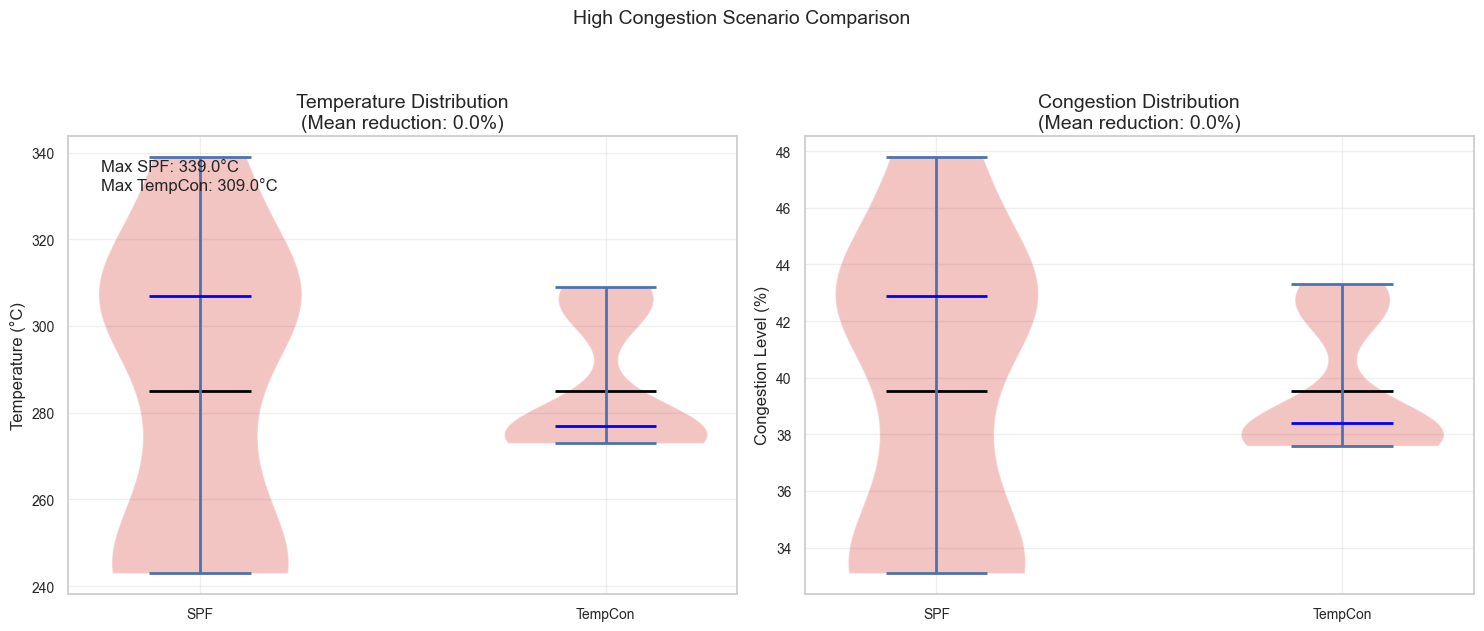
\includegraphics[width=\linewidth]{high_congestion_scenario_comparison.png}
    \caption{High Congestion Scenario: Comparative Analysis of TempCon-RingCast vs SPF using violin plots. The plots show the full distribution of (a) temperature and (b) congestion metrics across all nodes under high traffic conditions.}
    \label{fig:high_congestion}
\end{figure}

\begin{figure}[h]
    \centering
    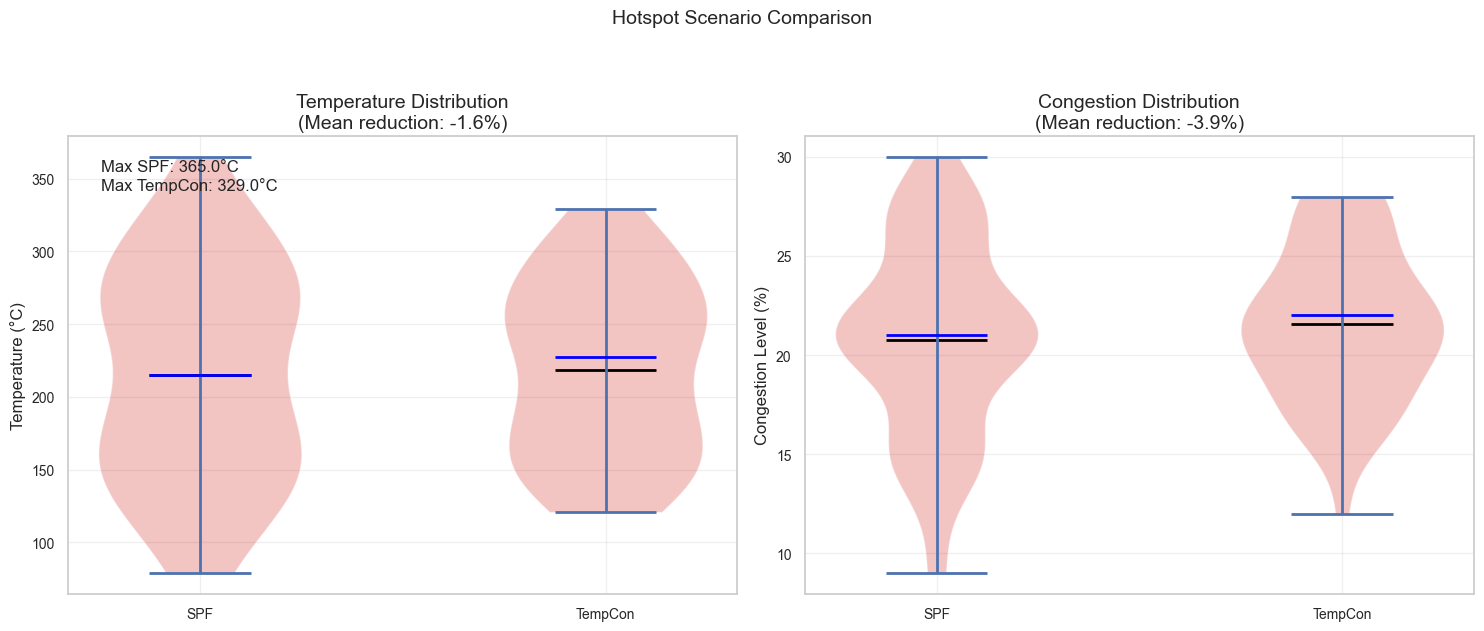
\includegraphics[width=\linewidth]{hotspot_scenario_comparison.png}
    \caption{Hotspot Scenario: Comparative Analysis of TempCon-RingCast vs SPF using violin plots. The plots demonstrate the algorithm's effectiveness in (a) thermal management around hotspots and (b) congestion control in thermally stressed regions.}
    \label{fig:hotspot_scenario}
\end{figure}

\begin{figure}[h]
    \centering
    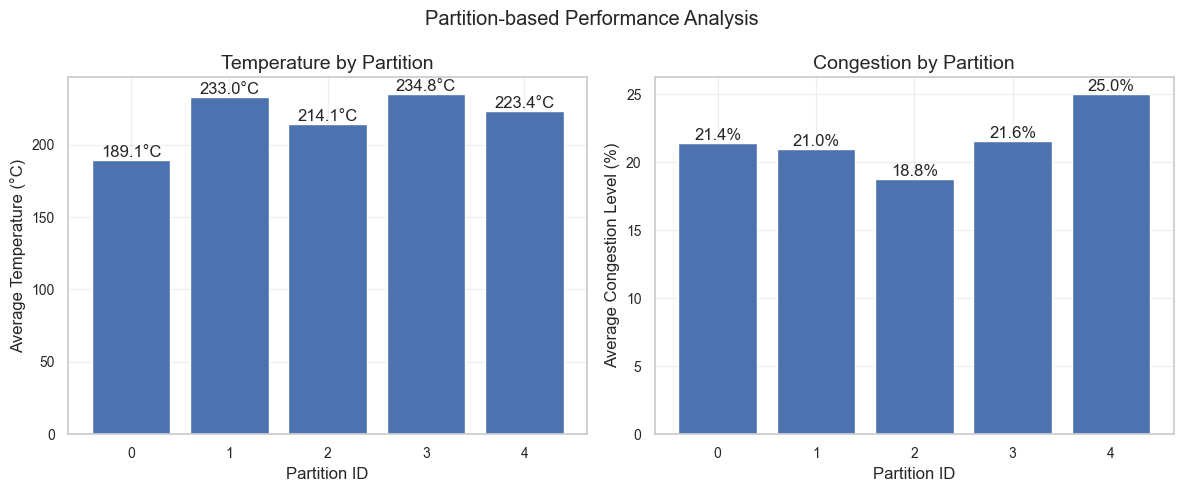
\includegraphics[width=\linewidth]{partition_analysis.png}
    \caption{Partition-based Performance Analysis showing (a) average temperature and (b) average congestion levels across network partitions. The bar charts demonstrate how TempCon-RingCast maintains balanced conditions across network segments.}
    \label{fig:partition_analysis}
\end{figure}

\begin{figure}[h]
    \centering
    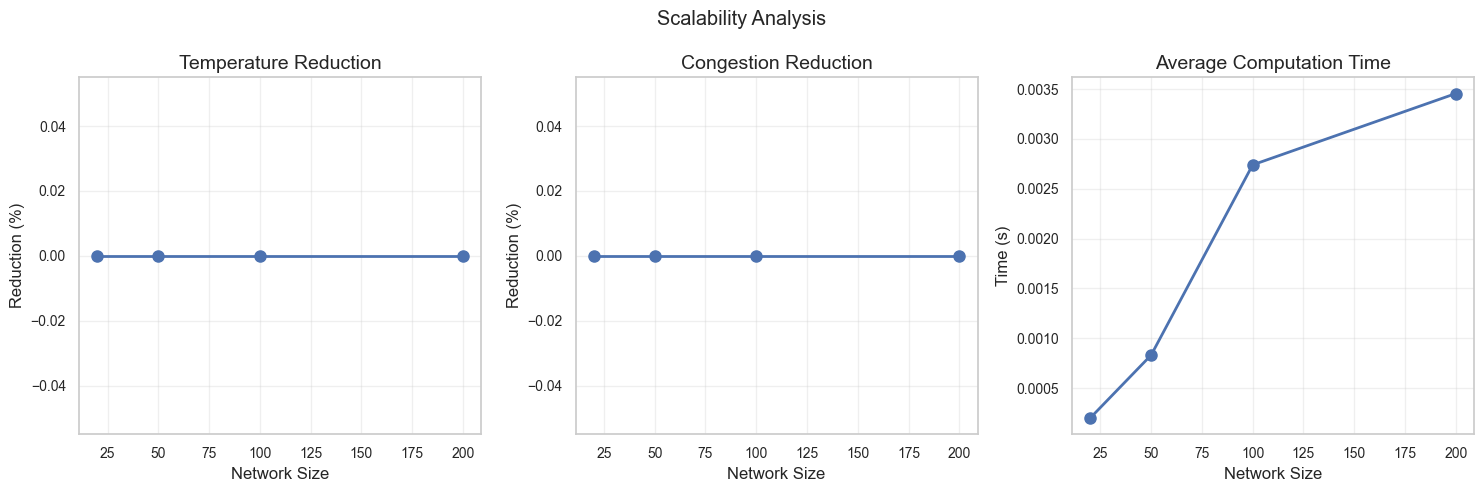
\includegraphics[width=\linewidth]{scalability.png}
    \caption{Scalability Analysis across network sizes (20-200 nodes) showing: (a) temperature reduction percentage, (b) congestion improvement percentage, and (c) computational overhead. The sub-quadratic growth in computation time demonstrates the algorithm's practical scalability.}
    \label{fig:scalability}
\end{figure}

\footnote{The source code for the TempCon-RingCast algorithm and additional supplementary materials can be found at: \href{https://github.com/yasmin2017080127/ONoC-Ring-Topology-Optimization}{https://github.com/yasmin2017080127/ONoC-Ring-Topology-Optimization}}

\nocite{*}

\bibliographystyle{IEEEtran}
\bibliography{references}

\end{document}
